\phantomsection
\chapter{Analysis}

The analysis was done while keeping several factors in mind. First of all, we had to compare the performance of the translation systems in consideration against that of prior translation systems. We also compared their performances with each other. To ensure the reliability of the automated metrics we compared them with the human scores, gaining interesting insights. We also assessed the change in performance in these systems with a change in sentence length. Finally, on the basis of scores obtained (human, as well as automated metric) we manually analyzed the translation by keeping them side by side to the reference sentences and listing the divergences and common errors that were observed from a linguistic perspective. Let's have a look at the results we obtained.

\phantomsection
\section{Sentence Length}

The first thing we analyzed was the sentence length, or the number of tokens in the sentence, the reference sentences, as well as the translated sentences. On preliminary observation, the data showed a degree of variability in the sentence length of the translated sentences in comparison to the corresponding reference sentences, a visual representation for the same can be seen in Fig \ref{fig:sen-len}.

\vspace{0.2cm}

\begin{figure}[h]
    \centering
    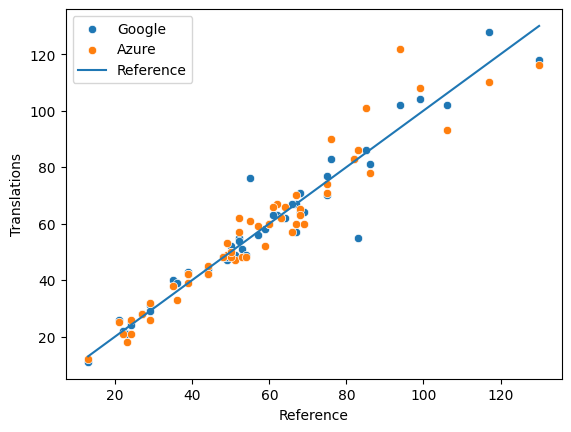
\includegraphics[width=0.8\linewidth]{images/sen_len.png}
    \caption{Length of Sentences}
    \label{fig:sen-len}
\end{figure}

As we can see, the spread of the data points validates our preliminary observation regarding the sentence length. Though this variability is low at shorter lengths, it increases with the increase in length. However, what surprised us the most was that though, we can see that there is a variability in the sentence length, the mean sentence length of the reference, and both the translation systems converge to a common length (see Table \ref{tab:sen-len})

\begin{center}    
\begin{table}[h]
\setlength\extrarowheight{5pt}
\centering
\begin{tabular}{p{4cm}@{}r}
    \textbf{Type} & \textbf{Length} \\
    \hline
    Reference & 57.86 \\
    Google & 57.82 \\
    Azure & 58.0
\end{tabular}
\caption{Mean Sentence Length}
\label{tab:sen-len}
\end{table}
\end{center}

\phantomsection
\section{Automated Metrics \& Human Scores}

Following this we looked at the scores obtained on different metrics, i.e., BLEU, ROUGE, and Human score. We have tabulated our the mean scores obtained for the aforementioned metrics below (see Table \ref{tab:score}).

\begin{center}
    \begin{table}[h]
    \setlength\extrarowheight{10pt}
        \centering
        \begin{tabular}{p{3cm}@{}p{3cm}@{}p{3cm}@{}c}
             & \textbf{Human} & \textbf{BLEU} & \textbf{ROUGE} \\
             \hline
            \textbf{Google} & 87.45 & 84.99 & [84.88, 70.32, 59.86, 79.81] \\
            \textbf{Azure} & 63.53 & 77.6 & [76.38, 56.21, 44.51, 68.22]
 \\ 
        \end{tabular}
        \caption{Mean scores obtained on different metrics}
        \label{tab:score}
    \end{table}
\end{center}

\begin{figure}[h]
    \centering
    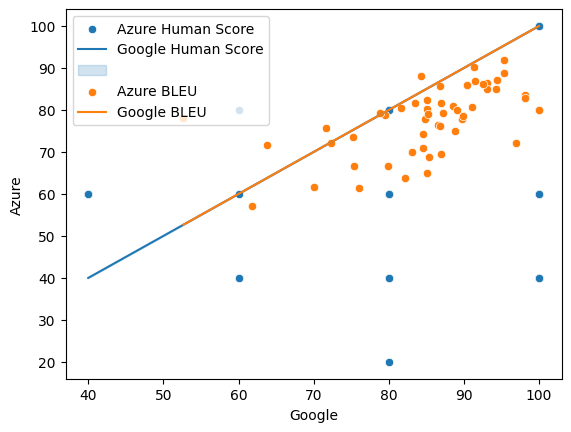
\includegraphics[width=0.9\linewidth]{images/human_bleu.png}
    \caption{Human vs BLEU scores}
    \label{fig:human-v-bleu}
\end{figure}

Table \ref{tab:score} shows a close correlation between the Human score, the BLEU score and the ROUGE-1 score for Google, which is also substantiated by Fig \ref{fig:human-v-bleu}. Even though the Human score is quite different for Azure, it still presents an interpretable picture of both the translation systems. The correlation with Human evaluation validates the BLEU score. BLEU score is usually within the range from 0 to 1, here we have obtained a converted BLEU score in the range of 0 to 100. A higher BLEU score signifies better translation performance. Both Google and Azure translate show a significant improvement when compared to the model Vaswani trained in the paper `\textit{Attention Is All You Need}' \cite{vaswani2017attention} back in 2017, the model had a BLEU score of 41.0.

\begin{figure}[h]
    \centering
    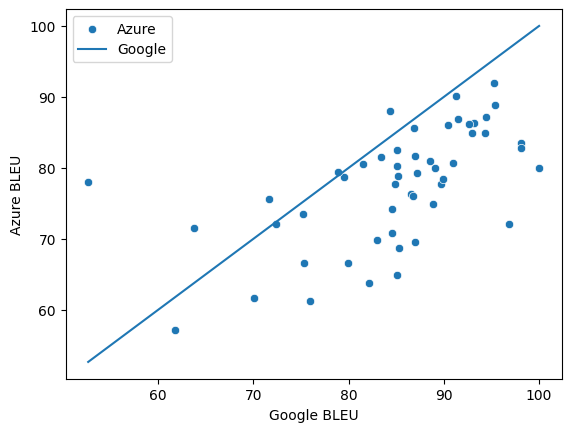
\includegraphics[width=0.9\linewidth]{images/bleu.png}
    \caption{Google vs Azure BLEU score}
    \label{fig:google-v-azure}
\end{figure}

From comparison we also observed that Google Translate performed better than Azure in all of the metrics, the Fig \ref{fig:google-v-azure} visually states the superiority in performance of Google Translate over Azure Translate. There are a few cases where Azure performs better than Google, but Google is the winner overall. This correlation is also supported by the ROUGE metric and the Human score as well Fig \ref{tab:score} Table \ref{tab:score}.

\phantomsection
\section{Manual Analysis}

Now to analyze the translations manually. The fluency of both the systems was remarkable, barely showing any signs of breaking the flow. Though Azure in a couple of cases showed severely improper translations for which the human evaluator assigned it a score of 1 (you can refer to the dataset uploaded online, Section 47, 52, 147, 444 etc.). 

\singlespacing
For Example: \underline{\textbf{Section 444}}
\begin{quote}
    \textbf{English Reference}: `\textit{Lurking house-trespass by night}'\\
    \textbf{Google Translate}: `\textit{Secret house-trespass at night}'\\
    \textbf{Azure Translate}: `\textit{Night Hidden Planet Trespass}'
\end{quote}
\doublespacing

In case of artificiality, there were barely such observations. The most commonly observed divergence were syntactic and lexical divergences, you could find one in almost every sentence. However, the equivalents presented were quite acceptable, except for in some cases. Let's take a look at few examples:-

\singlespacing
\underline{\textbf{Section 47}}
\begin{quote}
    \textbf{English Reference}: `\textit{“Animal”.—The word “animal” denotes any living creature, other than a human being.}'\\
    \textbf{Google Translate}: `\textit{Animal - The word animal denotes any living creature other than human.}'\\
    \textbf{Azure Translate}: `\textit{Fauna : The word animal denotes any living being other than human beings}'
\end{quote}

\underline{\textbf{Section 7}}
\begin{quote}
    \textbf{English Reference}: `\textit{Sense of expression once explained}'\\
    \textbf{Google Translate}: `\textit{Meaning of phrase once explained}'\\
    \textbf{Azure Translate}: `\textit{Meaning of a once clarified phrase}'
\end{quote}

\underline{\textbf{Section 465}}
\begin{quote}
    \textbf{English Reference}: `\textit{Punishment for forgery}'\\
    \textbf{Google Translate}: `\textit{Punishment for forgery}'\\
    \textbf{Azure Translate}: `\textit{Penalty for encryption}'
\end{quote}
\doublespacing

Some of the lexical divergences are acceptable such as in Section 7, while some cause some confusion about the overall meaning of the utterance such as in Section 47. There are cases where there is a bit too much divergence as exemplified by Section 465, where `\textit{forgery}' is replaced by `\textit{encryption}'. There are also cases where these divergences cause the whole meaning of the utterance to be undecipherable, as shown in Section 444 above. There cases of other kinds of divergences as well, Section 7 shows syntactic divergence in case of Azure. Overall, there divergences are in the output of both translation systems. However, in case of Google they are less frequent and mostly acceptable, whereas in case of Azure these divergences are not only frequent but also cause a loss of sense and coherence of the source utterance. The observations seem to correlate with the scores.